%%
% Copyright (c) 2017 - 2022, Pascal Wagler;
% Copyright (c) 2014 - 2022, John MacFarlane
%
% All rights reserved.
%
% Redistribution and use in source and binary forms, with or without
% modification, are permitted provided that the following conditions
% are met:
%
% - Redistributions of source code must retain the above copyright
% notice, this list of conditions and the following disclaimer.
%
% - Redistributions in binary form must reproduce the above copyright
% notice, this list of conditions and the following disclaimer in the
% documentation and/or other materials provided with the distribution.
%
% - Neither the name of John MacFarlane nor the names of other
% contributors may be used to endorse or promote products derived
% from this software without specific prior written permission.
%
% THIS SOFTWARE IS PROVIDED BY THE COPYRIGHT HOLDERS AND CONTRIBUTORS
% "AS IS" AND ANY EXPRESS OR IMPLIED WARRANTIES, INCLUDING, BUT NOT
% LIMITED TO, THE IMPLIED WARRANTIES OF MERCHANTABILITY AND FITNESS
% FOR A PARTICULAR PURPOSE ARE DISCLAIMED. IN NO EVENT SHALL THE
% COPYRIGHT OWNER OR CONTRIBUTORS BE LIABLE FOR ANY DIRECT, INDIRECT,
% INCIDENTAL, SPECIAL, EXEMPLARY, OR CONSEQUENTIAL DAMAGES (INCLUDING,
% BUT NOT LIMITED TO, PROCUREMENT OF SUBSTITUTE GOODS OR SERVICES;
% LOSS OF USE, DATA, OR PROFITS; OR BUSINESS INTERRUPTION) HOWEVER
% CAUSED AND ON ANY THEORY OF LIABILITY, WHETHER IN CONTRACT, STRICT
% LIABILITY, OR TORT (INCLUDING NEGLIGENCE OR OTHERWISE) ARISING IN
% ANY WAY OUT OF THE USE OF THIS SOFTWARE, EVEN IF ADVISED OF THE
% POSSIBILITY OF SUCH DAMAGE.
%%

%%
% This is the Eisvogel pandoc LaTeX template.
%
% For usage information and examples visit the official GitHub page:
% https://github.com/Wandmalfarbe/pandoc-latex-template
%%

% Options for packages loaded elsewhere
\PassOptionsToPackage{unicode}{hyperref}
\PassOptionsToPackage{hyphens}{url}
\PassOptionsToPackage{dvipsnames,svgnames,x11names,table}{xcolor}
%
\documentclass[
  paper=a4,
  ,captions=tableheading
]{scrartcl}
\usepackage{amsmath,amssymb}
% Use setspace anyway because we change the default line spacing.
% The spacing is changed early to affect the titlepage and the TOC.
\usepackage{setspace}
\setstretch{1.2}
\usepackage{iftex}
\ifPDFTeX
  \usepackage[T1]{fontenc}
  \usepackage[utf8]{inputenc}
  \usepackage{textcomp} % provide euro and other symbols
\else % if luatex or xetex
  \usepackage{unicode-math} % this also loads fontspec
  \defaultfontfeatures{Scale=MatchLowercase}
  \defaultfontfeatures[\rmfamily]{Ligatures=TeX,Scale=1}
\fi
\usepackage{lmodern}
\ifPDFTeX\else
  % xetex/luatex font selection
\fi
% Use upquote if available, for straight quotes in verbatim environments
\IfFileExists{upquote.sty}{\usepackage{upquote}}{}
\IfFileExists{microtype.sty}{% use microtype if available
  \usepackage[]{microtype}
  \UseMicrotypeSet[protrusion]{basicmath} % disable protrusion for tt fonts
}{}
\makeatletter
\@ifundefined{KOMAClassName}{% if non-KOMA class
  \IfFileExists{parskip.sty}{%
    \usepackage{parskip}
  }{% else
    \setlength{\parindent}{0pt}
    \setlength{\parskip}{6pt plus 2pt minus 1pt}}
}{% if KOMA class
  \KOMAoptions{parskip=half}}
\makeatother
\usepackage{xcolor}
\definecolor{default-linkcolor}{HTML}{A50000}
\definecolor{default-filecolor}{HTML}{A50000}
\definecolor{default-citecolor}{HTML}{4077C0}
\definecolor{default-urlcolor}{HTML}{4077C0}
\usepackage[margin=2.5cm,includehead=true,includefoot=true,centering,]{geometry}
% add backlinks to footnote references, cf. https://tex.stackexchange.com/questions/302266/make-footnote-clickable-both-ways
\usepackage{footnotebackref}
\usepackage{graphicx}
\makeatletter
\def\maxwidth{\ifdim\Gin@nat@width>\linewidth\linewidth\else\Gin@nat@width\fi}
\def\maxheight{\ifdim\Gin@nat@height>\textheight\textheight\else\Gin@nat@height\fi}
\makeatother
% Scale images if necessary, so that they will not overflow the page
% margins by default, and it is still possible to overwrite the defaults
% using explicit options in \includegraphics[width, height, ...]{}
\setkeys{Gin}{width=\maxwidth,height=\maxheight,keepaspectratio}
% Set default figure placement to htbp
\makeatletter
\def\fps@figure{htbp}
\makeatother
\setlength{\emergencystretch}{3em} % prevent overfull lines
\providecommand{\tightlist}{%
  \setlength{\itemsep}{0pt}\setlength{\parskip}{0pt}}
\setcounter{secnumdepth}{5}
\usepackage{booktabs}
\usepackage{longtable}
\usepackage{array}
\usepackage{multirow}
\usepackage{wrapfig}
\usepackage{float}
\usepackage{colortbl}
\usepackage{pdflscape}
\usepackage{tabu}
\usepackage{threeparttable}
\usepackage{threeparttablex}
\usepackage[normalem]{ulem}
\usepackage{makecell}
\usepackage{xcolor}
\ifLuaTeX
  \usepackage{selnolig}  % disable illegal ligatures
\fi
\IfFileExists{bookmark.sty}{\usepackage{bookmark}}{\usepackage{hyperref}}
\IfFileExists{xurl.sty}{\usepackage{xurl}}{} % add URL line breaks if available
\urlstyle{same}
\hypersetup{
  pdftitle={Diamonds},
  pdfauthor={Francisco Arrieta, Emily Schmidt and Lucia Camenisch},
  hidelinks,
  breaklinks=true,
  pdfcreator={LaTeX via pandoc with the Eisvogel template}}
\title{Diamonds}
\author{Francisco Arrieta, Emily Schmidt and Lucia Camenisch}
\date{2022-12-20}



%%
%% added
%%


%
% for the background color of the title page
%
\usepackage{pagecolor}
\usepackage{afterpage}
\usepackage[margin=2.5cm,includehead=true,includefoot=true,centering]{geometry}

%
% break urls
%
\PassOptionsToPackage{hyphens}{url}

%
% When using babel or polyglossia with biblatex, loading csquotes is recommended
% to ensure that quoted texts are typeset according to the rules of your main language.
%
\usepackage{csquotes}

%
% captions
%
\definecolor{caption-color}{HTML}{777777}
\usepackage[font={stretch=1.2}, textfont={color=caption-color}, position=top, skip=4mm, labelfont=bf, singlelinecheck=false, justification=raggedright]{caption}
\setcapindent{0em}

%
% blockquote
%
\definecolor{blockquote-border}{RGB}{221,221,221}
\definecolor{blockquote-text}{RGB}{119,119,119}
\usepackage{mdframed}
\newmdenv[rightline=false,bottomline=false,topline=false,linewidth=3pt,linecolor=blockquote-border,skipabove=\parskip]{customblockquote}
\renewenvironment{quote}{\begin{customblockquote}\list{}{\rightmargin=0em\leftmargin=0em}%
\item\relax\color{blockquote-text}\ignorespaces}{\unskip\unskip\endlist\end{customblockquote}}

%
% Source Sans Pro as the de­fault font fam­ily
% Source Code Pro for monospace text
%
% 'default' option sets the default
% font family to Source Sans Pro, not \sfdefault.
%
\ifnum 0\ifxetex 1\fi\ifluatex 1\fi=0 % if pdftex
    \usepackage[default]{sourcesanspro}
  \usepackage{sourcecodepro}
  \else % if not pdftex
    \usepackage[default]{sourcesanspro}
  \usepackage{sourcecodepro}

  % XeLaTeX specific adjustments for straight quotes: https://tex.stackexchange.com/a/354887
  % This issue is already fixed (see https://github.com/silkeh/latex-sourcecodepro/pull/5) but the
  % fix is still unreleased.
  % TODO: Remove this workaround when the new version of sourcecodepro is released on CTAN.
  \ifxetex
    \makeatletter
    \defaultfontfeatures[\ttfamily]
      { Numbers   = \sourcecodepro@figurestyle,
        Scale     = \SourceCodePro@scale,
        Extension = .otf }
    \setmonofont
      [ UprightFont    = *-\sourcecodepro@regstyle,
        ItalicFont     = *-\sourcecodepro@regstyle It,
        BoldFont       = *-\sourcecodepro@boldstyle,
        BoldItalicFont = *-\sourcecodepro@boldstyle It ]
      {SourceCodePro}
    \makeatother
  \fi
  \fi

%
% heading color
%
\definecolor{heading-color}{RGB}{40,40,40}
\addtokomafont{section}{\color{heading-color}}
% When using the classes report, scrreprt, book,
% scrbook or memoir, uncomment the following line.
%\addtokomafont{chapter}{\color{heading-color}}

%
% variables for title, author and date
%
\usepackage{titling}
\title{Diamonds}
\author{Francisco Arrieta, Emily Schmidt and Lucia Camenisch}
\date{2022-12-20}

%
% tables
%

%
% remove paragraph indention
%
\setlength{\parindent}{0pt}
\setlength{\parskip}{6pt plus 2pt minus 1pt}
\setlength{\emergencystretch}{3em}  % prevent overfull lines

%
%
% Listings
%
%


%
% header and footer
%
\usepackage[headsepline,footsepline]{scrlayer-scrpage}

\newpairofpagestyles{eisvogel-header-footer}{
  \clearpairofpagestyles
  \ihead*{Diamonds}
  \chead*{}
  \ohead*{2022-12-20}
  \ifoot*{Francisco Arrieta, Emily Schmidt and Lucia Camenisch}
  \cfoot*{}
  \ofoot*{\thepage}
  \addtokomafont{pageheadfoot}{\upshape}
}
\pagestyle{eisvogel-header-footer}



%%
%% end added
%%

%% adding more size options for the title
\usepackage{moresize}

\begin{document}

%%
%% begin titlepage
%%
\begin{titlepage}
\newgeometry{left=6cm}
\newcommand{\colorRule}[3][black]{\textcolor[HTML]{#1}{\rule{#2}{#3}}}
\begin{flushleft}
\noindent
\\[-1em]
\color[HTML]{5F5F5F}
\makebox[0pt][l]{\colorRule[FFFFFF]{1.3\textwidth}{4pt}}
\par
\noindent

{
  \setstretch{1.4}
  \vfill
  \noindent {\huge \textbf{\textsf{Diamonds}}}
    \vskip 2em
  \noindent {\Large \textsf{Francisco Arrieta, Emily Schmidt and Lucia
Camenisch}}
  \vfill
}


\textsf{2022-12-20}
\end{flushleft}
\end{titlepage}
\restoregeometry
\pagenumbering{arabic} 

%%
%% end titlepage
%%

% \maketitle


{
\setcounter{tocdepth}{3}
\tableofcontents
}
\hypertarget{introduction}{%
\section{Introduction}\label{introduction}}

The following report provides the result of using machine learning as a
tool to estimate diamond prices for a jewelry company. Using snapshot
information from their asset database, various methods were applied to
train predictive models using regression analysis. The main objective
was to use supervised learning methods to predict prices. These models
are later compared to measure their effectiveness by using error
measurements to quantify the distance between the prediction and the
actual price. Finally, conclusions on the capability of each model are
made and suggestions are given on which model to apply for the problem
at hand.

The product being analyzed is diamonds. Being a luxury object with a
long history, industry standards have been developed to serve as
guidelines for estimating the value of the product. A wide variety of
characteristics affect the overall price of diamonds, but this analysis
will focus on their physical qualities, such as size dimensions, size
ratios and color. Other factors inherent to scarce products in high
demand of a capitalist economy will not be considered in our machine
learning exercise.

The choice of methods shown in the report is not all inclusive and
responds to the fact of only being some of the most used methods to this
day. By implementing them, the analysts hope to provide a glimpse of the
effects and importance in choosing the right model as well as displaying
the differences between each one.

\hypertarget{data-exploration}{%
\section{Data Exploration}\label{data-exploration}}

In the early stages of any analysis, data exploration is a critical
process aimed at understanding and analyzing the data set to gain
insight and make valid decisions. The overarching goal of examining the
data is to obtain intuition, identify questionable values, and
strategize how to answer the problem statement. Therefore, let's
summarize the findings that explain the main data characteristics, and
dive into the relations between variables to understand how this
analysis will be directed.

\hypertarget{dimension-summary}{%
\subsection{Dimension Summary}\label{dimension-summary}}

There is a variety of ways an analyst could approach understanding the
observations in the data set. For starters, there are 53,940 records and
10 variables. The response variable (price) is a an integer variable.
There are an additional six numeric values and three ordinal/categorical
features that have a factored structure. Those non-numeric values
(\texttt{cut}, \texttt{color}, and \texttt{clarity}) need to be
appropriately ordered, and renamed if there are any spaces within their
naming convention as later this could obstruct certain code.

To dive deeper, we consider removing observations that are invalid
because they add noise. For instance, price against all features were
reviewed for possible impurities. In total, there are 275 (0.5\%)
records removed for the following reasons:

\begin{enumerate}
\def\labelenumi{\arabic{enumi}.}
\item
  20 rows had a depth of 0.0. This was considered inaccurate because a
  diamond needs to have this dimension specified.
\item
  The difference between length and width should be almost identical. If
  they were not, those rows were removed. In this case, only two records
  were not included in the data set at differences above 36.0mm.
\item
  The depth\_ratio is a calculation between length, width, and length.
  To investigate this feature further, our group computed depth\_ratio
  and saw there were differences between the actual and predicted
  values. Therefore, the executive decision was to remove any
  differences above a threshold of 0.3. A total of 253 rows were
  removed.
\end{enumerate}

Fortunately, there were no null values that needed to be considered.

\begin{center}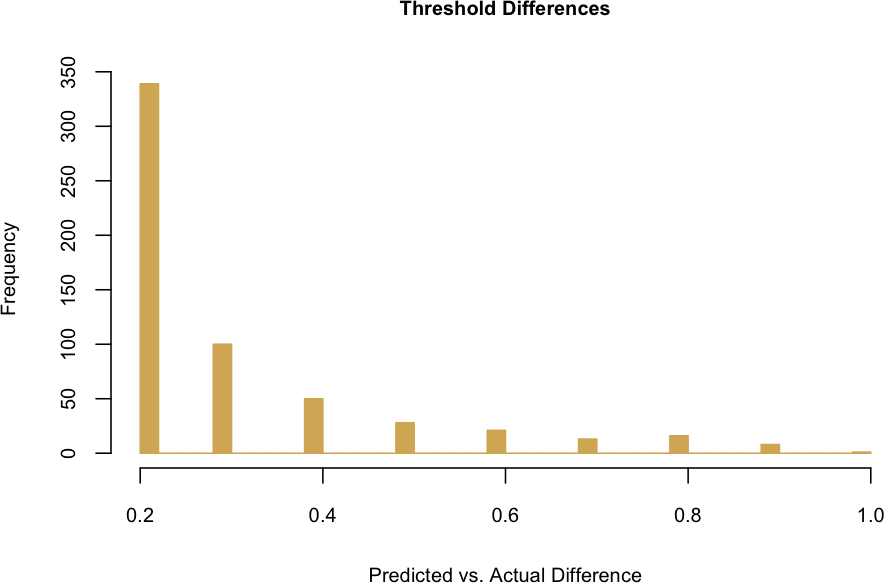
\includegraphics{Diamonds_PDF_files/figure-latex/threshold diff hist-1} \end{center}

The second part of exploring the diamonds data set is to understand the
relationships between variables. Prior to analyzing their correlations,
we had an idea of which continuous variables would have a strong
relation due to the depth\_ratio calculation. Later on, certain methods
will analyze the potential issue of collinearity. By isolating price
against the other continuous variables, carat, length, width, and depth,
all have positively linear relations to the response feature. Some of
the models used in the analysis to predict price will show these
effects. In addition, the relationship between carat and price is unique
because their relation is non-linear. We were also interested in showing
how the categorical variables affect price. Clarity, color, and cut have
distinct patterns seen between the four continuous variables mentioned
above.

For instance, when plotting price by carat, width, length, and depth,
with clarity as the color dimension, there is a clear distinction
between how these points relate. Each scatter plot shows a strong,
positive correlation to price. When reviewing the x-axis for each
explanatory variable, the lower tiered option is typically observed
more. The cheaper the gemstone, the worse quality the customer bought.
Within each plot, there are outliers that can be explained by how the
diamond was cut, which impacts the weight, length, and depth. By the
color scale, it is noticed how there are more diamonds with a worse
clarity (SI2/SI1) than there are with the best (IF/VVS1). Intuitively,
this makes sense because not all customers have the available funds to
afford the optimally designed diamond. On the other hand, no one wants
the worst clarity either. Therefore, a majority of the diamonds lie
between the second and third best, and second and third worst clarity
factors. In addition, the relation between depth\_ratio and table to
price is not distinct as those features are mixed throughout the
relative ranges. Within all of the depth\_ratio plots, there are
vertical lines that show the depth\_ratio mean (black) and range (red)
of what is considered the prime value for depth\_ratio as long as it is
above 59\% but does not exceed 62.3\%.

\begin{center}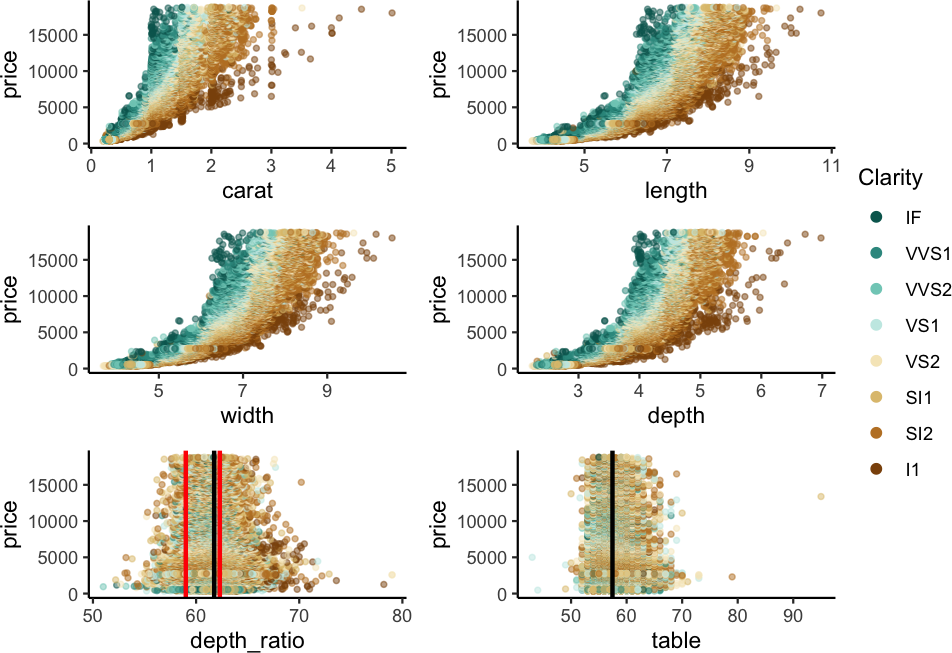
\includegraphics{Diamonds_PDF_files/figure-latex/Price by X and Clarity-1} \end{center}

A similar relationship can be seen regarding price by the continuous
variables, but as color as the color dimension. Instead of most of the
observations falling closer to the best and worth clarify features, here
the reader will notice how it appears that the colors E, F and G
dominate (the white to light blue) the retail space.

\begin{center}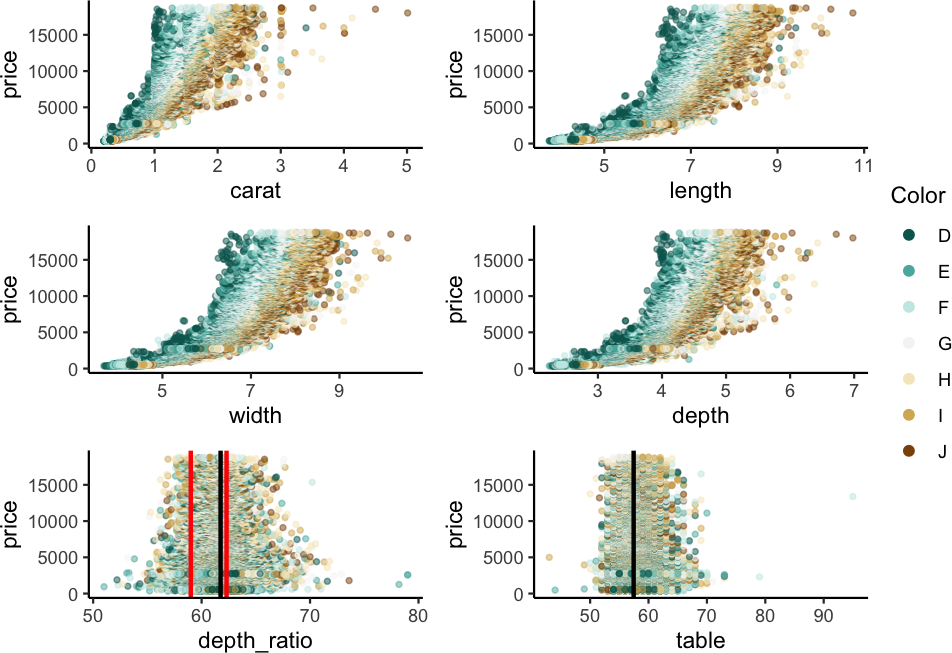
\includegraphics{Diamonds_PDF_files/figure-latex/Price by X and Color-1} \end{center}

Cut has a completely different trend than clarity and color as a
majority of customers prefer and will purchase the ideal cut. This can
be seen within the depth\_ratio plot especially. As stated earlier, the
red lines indicate the optimal space in which a buyer would want the
diamond's depth\_ratio. Most of all of the ideal cuts are within those
bounds while the fair, good, and very good are outside. There is a clear
distinction on how cut relates to the depth\_ratio along price.

\begin{center}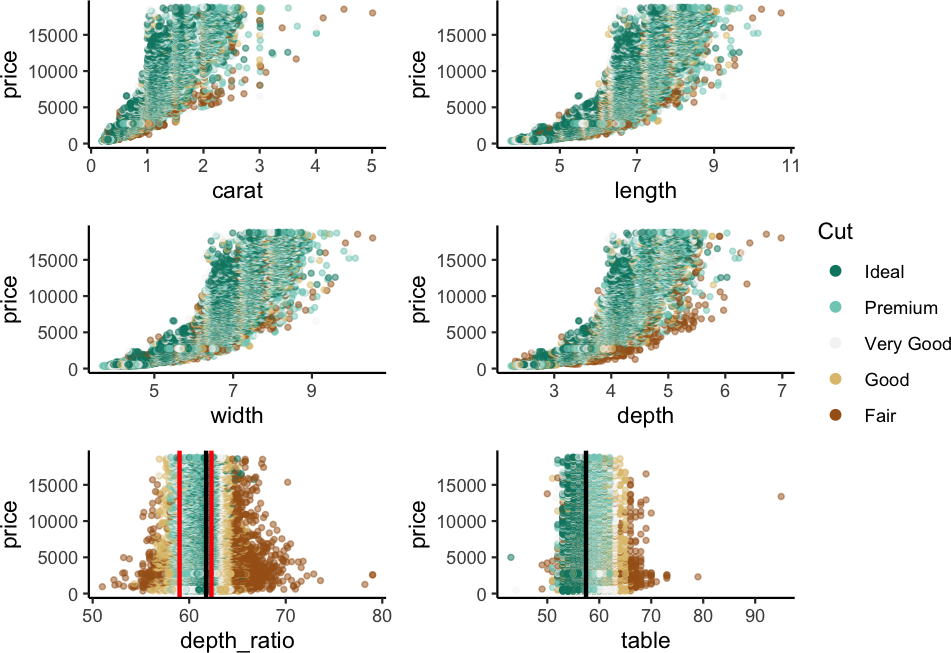
\includegraphics{Diamonds_PDF_files/figure-latex/Price by X and Cut-1} \end{center}

\hypertarget{variable-visualisation}{%
\subsection{Variable Visualisation}\label{variable-visualisation}}

As a continuation of data exploration, variable visualization involves
creating graphical representations of data to visually communicate
insights and trends. It allows us to quickly and easily identify
patterns that may not be immediately apparent from looking at raw data.
There are three graphics that demonstrate how these continuous values
are distributed. Since some models take into account transformation,
those details will be described later. As a high-level overview, price
and carat are positively skewed. In the scatter plot regarding price by
cut for the depth\_ratio, the histogram also displays the same
conclusion that the cut features fall into approximately 60 to 65 mm.
The relationships in the Correlation heat map visually show how width,
length, depth, and carat continue to be highly correlated with price
while depth\_ratio and table are closer to 0. Another way to visualize
the relationships is through the Pearson Correlation Ellipses chart. The
skinnier the ellipse, the more correlated the two values are.

Through exploration, we can gain a deeper understanding of the data and
how it can be used to answer business questions or solve real-world
problems, like predicting the price of a diamond.

\begin{center}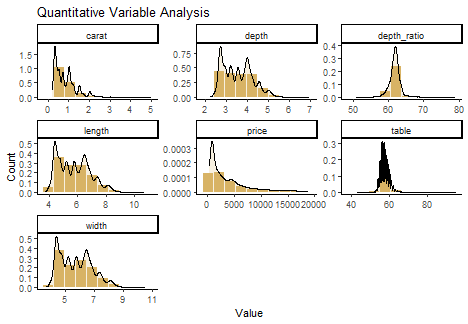
\includegraphics{Diamonds_PDF_files/figure-latex/Histograms-1} \end{center}

\begin{center}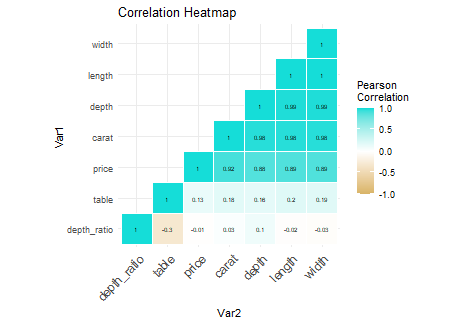
\includegraphics{Diamonds_PDF_files/figure-latex/Correlation-1} \end{center}

\hypertarget{variable-prediction-and-model-performance-evaluation}{%
\section{Variable Prediction and Model Performance
Evaluation}\label{variable-prediction-and-model-performance-evaluation}}

\hypertarget{linear-regression}{%
\subsection{Linear Regression}\label{linear-regression}}

\hypertarget{data-preparation}{%
\subsubsection{Data preparation}\label{data-preparation}}

We begin by performing linear regressions on our data. As we saw during
the exploration phase, some predictors (\texttt{carat}, \texttt{length},
\texttt{width} and \texttt{depth}) are highly correlated. Therefore,
multicollinearity might be an issue.

We use the Generalized Variation Inflation Factors (GVIF) to measure the
multicollinearity level of our data. This generalized version of the VIF
allows us to take into account numerical and categorical predictors
together. The GVIF clearly confirms that there is an issue, as
\texttt{length}, \texttt{width} and \texttt{depth} all have coefficients
above 1000. \texttt{carat} and \texttt{depth\_ratio} also have high
values above 25, but they aren't as high extreme as the other three.

After removing \texttt{length}, \texttt{width} and \texttt{depth}, the
GVIF coefficients of the remaining predictors are all under 2, which
indicates the multicollinearity problem is solved. We display
correlation ellipses of numerical variables without \texttt{length},
\texttt{width} and \texttt{depth}.

\begin{center}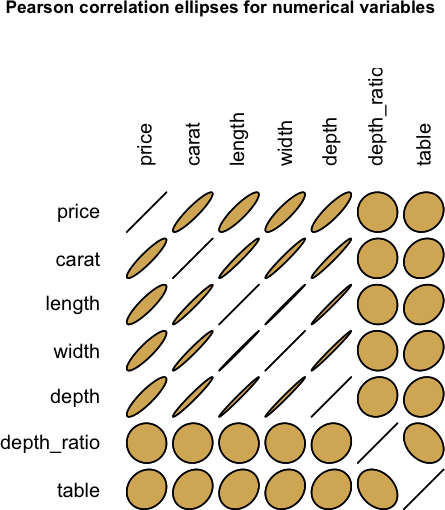
\includegraphics{Diamonds_PDF_files/figure-latex/uncorrelated-ellipses-1} \end{center}

The only high correlation left is between \texttt{carat} and
\texttt{price}, indicating that \texttt{carat} will surely be an
important predictor for determining \texttt{price}.

Thus, we will perform linear regressions on two different models:

\begin{enumerate}
\def\labelenumi{\arabic{enumi}.}
\tightlist
\item
  \texttt{LM\_complete} which contains all predictors
\item
  \texttt{LM\_minus\_corr} which has \texttt{length}, \texttt{width} and
  \texttt{depth} removed.
\end{enumerate}

These two models will serve as basis for variable selection procedures
later.

However, before starting to build our models, we also need to account
for skewed variables. Linear regression might perform worse when dealing
with skewed variables and it is common to use transformations such as a
logarithm or a \(n\)th root to make variable more symmetrical.

We use an estimator of skewness called \$b\_1\$, whose definition can be
found
\href{https://en.wikipedia.org/wiki/Skewness\#Sample_skewness}{here}.

The value of \(b_1\) is interpreted as follows:

\begin{itemize}
\tightlist
\item
  \(0 \leq |b_1| < 0.5\): variable is symmetrical;
\item
  \(0.5 \leq |b_1| < 1\): variable is moderately skewed;
\item
  \(|b_1| \geq 1\): variable is highly skewed.
\end{itemize}

We compute \(b_1\) on our numerical variables and get the following
results.

\begin{table}

\caption{\label{tab:skewness-table}Skewness estimator for numerical variables}
\centering
\begin{tabular}[t]{l|r}
\hline
  & \$b\_1\$\\
\hline
price & 1.6259747\\
\hline
carat & 1.0967514\\
\hline
length & 0.3984689\\
\hline
width & 0.3922008\\
\hline
depth & 0.3921093\\
\hline
depth\_ratio & 0.0182498\\
\hline
table & 0.8728869\\
\hline
\end{tabular}
\end{table}

\texttt{price} and \texttt{carat} are highly skewed and \texttt{table}
is moderately skewed.

We apply a logarithmic transformation to all three variables. The
improvement can also be seen in the histograms, as they look more
symmetrical now.

\begin{center}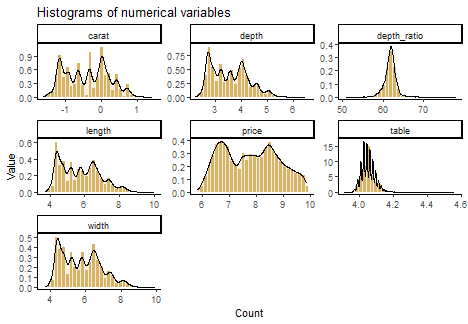
\includegraphics{Diamonds_PDF_files/figure-latex/hist-unskewed-1} \end{center}

We also standardize numerical variables by subtracting their mean and
dividing by their standard deviation. This makes the comparison of
\(\beta\) coefficients between variables easier.

\hypertarget{linear-models-based-on-complete-set-of-predictors}{%
\subsubsection{Linear models based on complete set of
predictors}\label{linear-models-based-on-complete-set-of-predictors}}

The data is now ready for our linear models. For both
\texttt{LM\_complete} and \texttt{LM\_minus\_corr}, we perform the
following linear regressions:

\begin{enumerate}
\def\labelenumi{\arabic{enumi}.}
\tightlist
\item
  Linear regression on the whole model
\item
  Forward selection on the model (iterative method)
\item
  Backward selection on the model (iterative method)
\item
  Stepwise selection on the model (iterative method)
\item
  Mallows's \(C_p\) and AIC selection on the model (global method)
\end{enumerate}

\hypertarget{linear-models-based-on-uncorrelated-predictors}{%
\subsubsection{Linear models based on uncorrelated
predictors}\label{linear-models-based-on-uncorrelated-predictors}}

\hypertarget{summary-of-models}{%
\subsubsection{Summary of models}\label{summary-of-models}}

For each of these models, we summarise which variables are used as
predictors in the following table.

\begin{table}

\caption{\label{tab:Variable Selection Summary}Predictors used in each linear model}
\centering
\begin{tabular}[t]{l|c|c|c|c|c|c|c|c|c}
\hline
Model & Cut & Color & Clarity & Carat & Length & Width & Depth & Depth Ratio & Table\\
\hline
LM\_complete & X & X & X & X & X & X & X & X & X\\
\hline
LM\_forward\_complete & X & X & X & X & X & X & X & X & X\\
\hline
LM\_backward\_complete & X & X & X & X & X &  & X & X & \\
\hline
LM\_stepwise\_complete & X & X & X & X & X &  & X & X & \\
\hline
LM\_CpAIC\_complete & X & X & X & X & X &  & X & X & \\
\hline
LM\_minus\_corr & X & X & X & X &  &  &  & X & X\\
\hline
LM\_forward\_minus\_corr & X & X & X & X &  &  &  & X & X\\
\hline
LM\_backward\_minus\_corr & X & X & X & X &  &  &  & X & \\
\hline
LM\_stepwise\_minus\_corr & X & X & X & X &  &  &  & X & \\
\hline
LM\_CpAIC\_minus\_corr & X & X & X & X &  &  &  & X & \\
\hline
\end{tabular}
\end{table}

For both basis models, forward selection doesn't discard any variables,
whereas backward, stepwise and global selections all choose the same
model with less variables than initially.

Thus, we have four distinct models in total. We assess the predictive
performance of these four models on our validation set by computing the
five accuracy measures seen during the course.

Let us recall the definitions and meaning of these measures (Data Mining
for Business Analytics - Concepts, Techniques, and Applications in R,
chapter 5.2, page 119). We denote the residuals by \(r = y - \hat y\).

\begin{enumerate}
\def\labelenumi{\arabic{enumi}.}
\tightlist
\item
  \textbf{ME} (Mean Error) gives an indication of whether the
  predictions are on average over- or under-predicting the outcome
  variable. \[ME = \dfrac{1}{n} \sum_{i=1}^{n}r_i\]
\item
  \textbf{RMSE} (Root Mean Squared Error) is similar to the standard
  error of estimate in linear regression, except that it is computed on
  the validation data rather than on the training data.
  \[RMSE =  \sqrt{\dfrac{1}{n}\sum_{i=1}^{n}r_i^2}\]
\item
  \textbf{MAE} (Mean Absolute Error) gives the magnitude of the average
  absolute error. \[MAE = \dfrac{1}{n} \sum_{i=1}^{n}|r_i|\]
\item
  \textbf{MPE} (Mean Percentage Error) gives the percentage score of how
  predictions deviate from the actual values (on average), taking into
  account the direction of the error.
  \[MPE = 100 \cdot \dfrac{1}{n} \sum_{i=1}^{n} \dfrac{r_i}{y_i}\]
\item
  \textbf{MAPE} (Mean Absolute Percentage Error) gives a percentage
  score of how predictions deviate (on average) from the actual values.
  \[MAPE = 100 \cdot \dfrac{1}{n} \sum_{i=1}^{n} \left| \dfrac{r_i}{y_i}\right|\]
\end{enumerate}

\hypertarget{accuracy-measures-of-models-on-validation-set}{%
\subsubsection{Accuracy measures of models on validation
set}\label{accuracy-measures-of-models-on-validation-set}}

The accuracy measures for our four models are summarized below. In order
to give meaningful results, the outcome variable \texttt{price} has been
rescaled to its original scale and retransformed by taking the
exponential (to cancel out the logarithm). Thus, the ME, RMSE and MAE
can be interpreted in the price currency, dollars.

\begin{table}

\caption{\label{tab:models-accuracy-table}Accuracy measures of linear models}
\centering
\begin{tabular}[t]{l|r|r|r|r|r}
\hline
Model & ME & RMSE & MAE & MPE & MAPE\\
\hline
LM\_complete & 36.36648 & 846.5888 & 408.5364 & -0.8377036 & 10.33643\\
\hline
LM\_CpAIC\_complete & 36.32774 & 845.5018 & 408.1349 & -0.8408540 & 10.33659\\
\hline
LM\_minus\_corr & 50.38994 & 810.1522 & 405.0486 & -0.8420621 & 10.39559\\
\hline
LM\_CpAIC\_minus\_corr & 50.39878 & 810.1610 & 405.0616 & -0.8418121 & 10.39568\\
\hline
\end{tabular}
\end{table}

The mean error is bigger in the models without multicollinearity issues,
but their RMSE is smaller. Since the mean error is positive in all four
models, we are under-predicting the price of diamonds by 36 or 50
dollars on average depending on the model.

An increase of 14\$ in the mean error is a good trade-off to reducing
the RMSE, which indicates how much the predictions will fluctuate from
real values. The other three measures are quite close in all four
models.

Considering the parsimony principle and the RMSE, the best choice is our
fourth linear model, which contains \texttt{cut}, \texttt{color},
\texttt{clarity}, \texttt{carat} and \texttt{depth\_ratio}.

Overall, the RMSE for linear regression remains quite high and as we
will see in the following chapters, some models will achieve much better
predictive performances.

\hypertarget{k-nn}{%
\subsection{\texorpdfstring{\(k\)-NN}{k-NN}}\label{k-nn}}

\hypertarget{overview}{%
\paragraph{Overview}\label{overview}}

\(k\)-nearest neighbors (kNN) is a simple algorithm used for
classification (categorical) and regression (continuous). Since the
response variable (price) is a numeric outcome, this analysis will use
\(k\)-NN to predict the price of a diamond. In a regression setting, the
algorithm relies on finding the most `similar' records in the training
data. Then, one would calculate the weighted average of the numerical
target of the \(k\)-nearest neighbors for the data point.

According to the Data Mining textbook, the value of k is based on a
nonparametric method since it `draws information from similarities
between the predictor values of the records in the dataset.' There are
several ways one could choose this hyperparameter, but this analysis
will focus on one method by the optimization of RMSE. k is a critical
input within the \(k\)-NN function because it determines how many
neighbors will be considered when making a prediction. Penn State states
that a `larger k leads to a smoother boundary but may also introduce
noise.' On the other side, a small k `can increase the complexity of
KNN.'

The \(k\)-nearest neighbors algorithm is very useful when predicting
price because the data does not need to be transformed or predictors
selected in a particular way.

\hypertarget{model-structure}{%
\paragraph{Model Structure}\label{model-structure}}

There are several steps that need to be completed prior to running the
first \(k\)-NN model with k = 1. First, you clean the data to ensure
that missing values are either removed or explained, and that all
variables are essential to the response variable (see EDA section).
Next, the data is normalized so that the output remains unbiased.
Normalizing simply means that the raw data is put on all the same scale
(`subtracting the mean and dividing by the standard deviation'). Once
the data is cleaned and normalized, it can be split into the training,
validation, and test sets. Now that the foundation of the model has been
built, let's start constructing the first \(k\)-NN model.

The value of k = 1 is used as a starting point to see how well the model
will perform. Since price is our focal point, the two error measurements
that will be compared throughout all model methods are Mean Error (ME)
and Root Mean Squared Error (RMSE). RMSE is of particular interest
because that gives the variance of how far the predicted value is away
from the actual price. Seen in the first \(k\)-NN error table, ME
(\$20.60) and RMSE (\$954.60) could potentially get better if we
optimized k.

The optimal k is 4 because it produces the lowest RMSE at \$814.59.
After rerunning the \(k\)-NN model, the results improved in one aspect,
but not the other.

\begin{tabu} to \linewidth {>{\raggedleft}X>{\raggedleft}X}
\hline
k & accuracy\\
\hline
1 & 954.5954\\
\hline
2 & 861.0887\\
\hline
3 & 827.1196\\
\hline
\cellcolor[HTML]{D8B365}{\textcolor{white}{\textbf{4}}} & \cellcolor[HTML]{D8B365}{\textcolor{white}{\textbf{814.5940}}}\\
\hline
5 & 819.2859\\
\hline
6 & 818.5541\\
\hline
7 & 822.7554\\
\hline
8 & 833.2104\\
\hline
9 & 839.9301\\
\hline
10 & 847.3985\\
\hline
11 & 850.7010\\
\hline
12 & 854.8280\\
\hline
13 & 860.4922\\
\hline
14 & 867.3541\\
\hline
15 & 874.8586\\
\hline
16 & 879.9069\\
\hline
17 & 886.0747\\
\hline
18 & 891.9780\\
\hline
19 & 896.3521\\
\hline
20 & 900.0938\\
\hline
\end{tabu}

\begin{center}\includegraphics{Diamonds_PDF_files/figure-latex/Best K Plot-1} \end{center}

\begin{table}
\centering
\begin{tabu} to \linewidth {>{\raggedright}X>{\raggedright}X>{\raggedright}X>{\raggedright}X>{\raggedright}X>{\raggedright}X}
\hline
  & ME & RMSE & MAE & MPE & MAPE\\
\hline
k = 1 & 20.6 & 954.6 & 487.17 & -1.83 & 13.73\\
\hline
k = 4 & 40.86 & 814.59 & 431.29 & -2.45 & 12.14\\
\hline
\end{tabu}
\end{table}

\begin{center}\includegraphics{Diamonds_PDF_files/figure-latex/knn error table-1} \end{center}

As stated earlier, the table above shows how the ME got worse for k = 4,
but better with RMSE once the model was optimized. In this analysis, one
of the main goals is to reduce the variance between predicted and real
price. Therefore, the difference of \$140.00 is more important even when
the ME slightly increases. Between k = 1 and k = 4 for the \(k\)-NN
model, k = 4 with an RMSE of \$814.60 will predict prices better.

\hypertarget{decision-trees}{%
\subsection{Decision Trees}\label{decision-trees}}

\hypertarget{regression-tree-overview}{%
\paragraph{Regression Tree Overview}\label{regression-tree-overview}}

There are four methods within this section that show various ways on how
trees are built. They include a regression tree, boosted tree, bagged
tree, and a random forest. The regression tree is most transparent and
easy to interpret while the other three combine results from multiple
trees.

A regression tree is a flexible data-driven method that can be used for
prediction of a continuous variable. The tree separates `records into
subgroups by creating splits on predictors. These splits create logical
rules that are homogeneous.' Those splits `divide the data into subsets,
that is, branches, nodes, and leaves. Like decision trees, regression
trees select splits that decrease the dispersion of target attribute
values. Thus, the target attribute values can be predicted from their
mean values in the leaves' which reduces the variance of the target
variable.

\hypertarget{model-structure-and-analysis}{%
\paragraph{Model Structure and
Analysis}\label{model-structure-and-analysis}}

Since the tree proactively takes into consideration the most important
attributes to split on, multiple trees are created to check its
validity. This idea stemmed from wanting to ensure that by removing
variables due to their weak relationship to the predictor variable or by
pruning, the results produced the best ME and RMSE. Within the three
regression models, all have the same error rates. In addition, there are
eight terminal nodes for each model and all had width, length, carat,
and depth being the most important features to predict price. To
exemplify this, we show the original regression tree that first splits
on width \textless{} 6.33, seven splits total and uses the following for
the primary splits: width \textless{} 6.325, carat \textless{} 0.985,
length \textless{} 6.325 and depth \textless{} 3.935.

\hypertarget{regression-tree}{%
\subsubsection{Regression Tree}\label{regression-tree}}

\begin{center}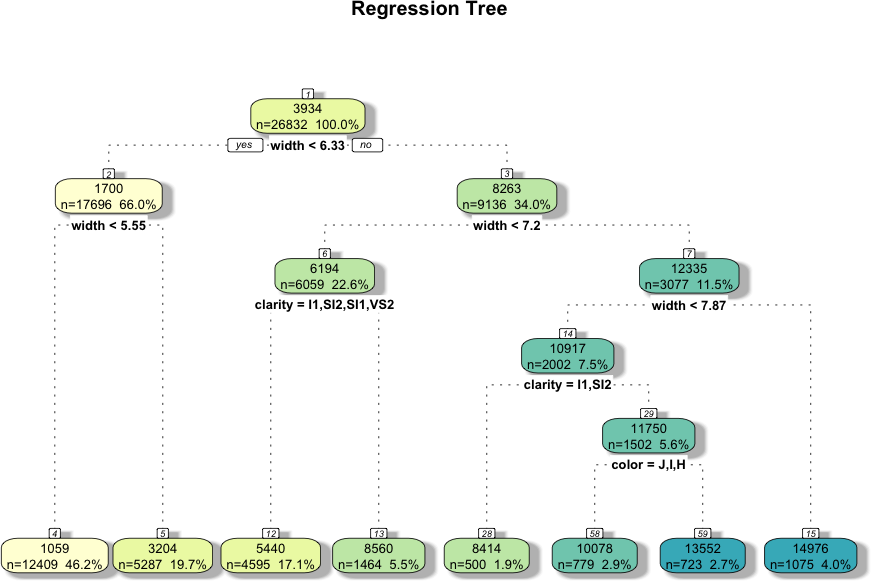
\includegraphics{Diamonds_PDF_files/figure-latex/Default Regression Tree-1} \end{center}

\hypertarget{boosted-tree}{%
\subsubsection{Boosted Tree}\label{boosted-tree}}

\hypertarget{overview-1}{%
\paragraph{Overview}\label{overview-1}}

Boosted trees are a type of ensemble model that `transforms weak
decision trees into strong learners. Each new tree is built considering
the errors of previous trees.' The idea behind boosting is to train a
series of weak models additively, with each model attempting to correct
the errors made by the previous model. Since this model is prone to
overfitting, the parameters need to be carefully considered so that the
lowest error rates can be achieved.

\hypertarget{model-structure-and-analysis-1}{%
\paragraph{Model Structure and
Analysis}\label{model-structure-and-analysis-1}}

There is a wide variety of parameters that can be chosen for a boosted
tree. Therefore, those options were used differently to choose the best
model based off the number of predictors and how deep each tree would be
allowed to interact. The main difference between each model is the
number of trees ran. As the size of the tree increase, the better the
model because it only considered the most important factors.

The best boosted model was the one with 100 trees and three
cross-validation folds. The tree used six predictors to produce a model
with a ME of \$9.00 and RMSE of \$1,170.30. What is fascinating about
this tree comes from the importance variables chart. In the regression
tree, clarity was one of the three least important factors, but here we
see that it as the fourth which is above length.

\hypertarget{bagged-tree}{%
\subsubsection{Bagged Tree}\label{bagged-tree}}

\hypertarget{overview-2}{%
\paragraph{Overview}\label{overview-2}}

The third method is bagged trees. This type of model `combines the
predictions from multiple machine learning algorithms together to make
more accurate predictions than any individual model.' The objective with
bagging is to train a large number of decision trees on different
subsets of the training data, and then average the predictions of all
the trees to make a final prediction. This model has the ability to
reduce variance because it introduces randomness into the training
process.

\hypertarget{model-structure-and-analysis-2}{%
\paragraph{Model Structure and
Analysis}\label{model-structure-and-analysis-2}}

This model is pretty straight forward because the best model was built
by sticking with the basics. `The only parameters when bagging decision
trees is the number of samples and hence the number of trees to include.
This can be chosen by increasing the number of trees on run after run
until the accuracy begins to stop showing improvement.' Overall, the
bagging tree predicts price better than the regression tree, but worse
than boosting. The ME was the lowest at \$0.93, but what is more
important to consider is the RMSE which is \$1,248.77.

\hypertarget{random-forest}{%
\subsubsection{Random Forest}\label{random-forest}}

\hypertarget{overview-3}{%
\paragraph{Overview}\label{overview-3}}

`Random forests are a special case of bagging, a method for improving
predictive power by combining multiple classifiers or prediction
algorithms.' They are an ensemble based on bagged trees which involves
training each tree on a bootstrapped sample of the original data.

\hypertarget{model-structure-1}{%
\paragraph{Model Structure}\label{model-structure-1}}

Similar to the bagged trees, random forests are pretty simplistic. The
main focus in this section was to check how many trees should be run
within the model. There is a trade-off between computational power and
RMSE. For example, what is the difference in RMSE if the model was built
off of 100 trees versus 60? The model with 100 trees was the best model
with an RMSE of \$575.42.

\begin{center}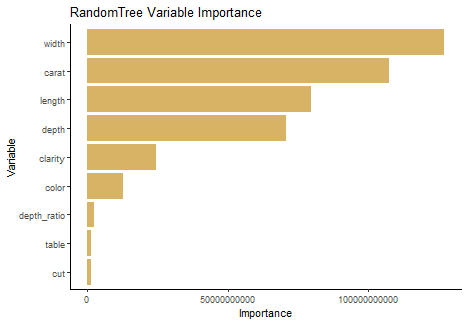
\includegraphics{Diamonds_PDF_files/figure-latex/RF Variable Importance-1} \end{center}

Throughout this entire section, typically the lower RMSE produced the
best model. Additionally up to this point, there have been three or four
variables that were most importance to the model. In the random forest
though, there is much more weight on features such as clarity and color.
In random forests, we proposed a trade-off with picking a model with
less trees because an analyst would want to choose the parsimonious
model. Therefore, the random forest with 60 trees had a slightly higher
RMSE at a difference of approximately \$2 which gave a \$577.63 for the
RMSE.

\hypertarget{decision-tree-summary-table}{%
\subsubsection{Decision Tree Summary
Table}\label{decision-tree-summary-table}}

\begin{table}
\centering
\begin{tabu} to \linewidth {>{\raggedright}X>{\raggedright}X>{\raggedright}X>{\raggedright}X>{\raggedright}X>{\raggedright}X}
\hline
  & ME & RMSE & MAE & MPE & MAPE\\
\hline
Reg. Tree & 6.1 & 1267.15 & 846.93 & -14.54 & 33.08\\
\hline
Exclus. RT & 6.1 & 1267.15 & 846.93 & -14.54 & 33.08\\
\hline
Pruned RT & 6.1 & 1267.15 & 846.93 & -14.54 & 33.08\\
\hline
Boost10 & -3.9 & 3660.42 & 2765.96 & -144.49 & 171.65\\
\hline
Boost30 & 2.54 & 1531.52 & 985.7 & -35.26 & 46.86\\
\hline
Boost100 & 9 & 1170.3 & 680.22 & -12.85 & 26.22\\
\hline
Bagging & 0.93 & 1248.77 & 808.93 & -14.35 & 31.45\\
\hline
RndmFrst & 2.97 & 577.63 & 289.51 & -1.4 & 7.24\\
\hline
\end{tabu}
\end{table}

\begin{center}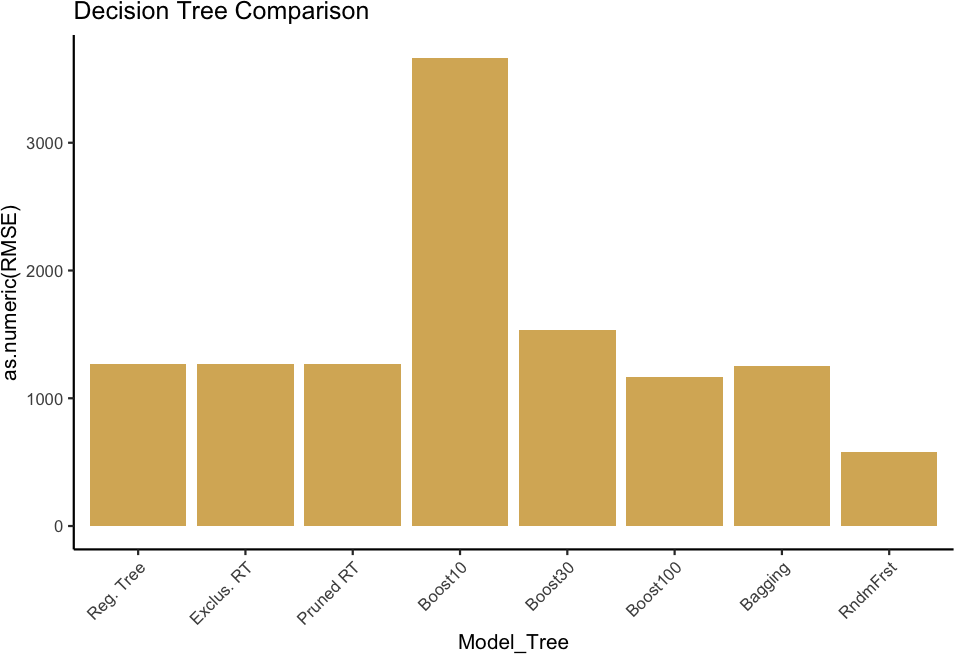
\includegraphics{Diamonds_PDF_files/figure-latex/RegTree Summary-1} \end{center}

Throughout the four methods mentioned, the random forest model proved to
be the most effective in predicting price with a RMSE of \$577.63, which
is more than two times smaller than the best boosting model. Although
not all of the models results are shown, a breakdown of their error
results can be seen within the table above. Overall, the regression
tree, bagging and boosting were all within \$100 RMSE difference, but no
match for the random forest.

\hypertarget{neuralnetworks}{%
\subsection{NeuralNetworks}\label{neuralnetworks}}

\hypertarget{basic-concept}{%
\subsubsection{Basic Concept}\label{basic-concept}}

Artificial neural networks are a method of machine learning that
receives the name due to a comparison made with actual neurons in the
human brain. They consist various nodes that communicate with each other
to predict an outcome based on the relationships that were determined in
the process. Neural nets have proven to be very good at predicting
values, through regression or classification and have been the center of
much research in the past years. Though this method was once considered
un useful, with the improvement of computational power, it has acquired
new popularity for prediction of images, speech recognition and
non-explicit trends. (Hardesty, 2017)

The basic parts of a neural networks are: the structure, composed of
layers and nodes, the weights, and the activation function. The first
consists of the different components used to train a neural network, ie
the explanatory variables and their connection. These independent
variables are considered the \emph{input nodes} and the outcome variable
the \emph{output node}. The layers in between these to are called the
\emph{hidden layers} as these are used to calculate the output but have
no easily association of there value with regards to the outcome. This
is why neural networks are considered by some like a \textbf{black box},
where the exact method for predicting is not easily explained to those
who are not well informed. The weights are used to pass a certain amount
of a value to the next node which after passing through the activation
function will pass on to the next, and so on. This weighting can be
assigned randomly or by specific methods, depending on the problem at
hand and analyst discretion. Similarly, the activation function
calculates the position in a curve, ie the expected value of the
prediction. This as well changes per prediction problem and analyst
discretion. While some are considered better for certain tasks there is
no limiting factor in the way a neural net is structured.

\hypertarget{data-preprocessing}{%
\subsubsection{Data preprocessing}\label{data-preprocessing}}

Due to the fact that in every node we calculate the position of the
prediction in a curve, the scale of the values used affects the output
of every node. Moreover, since we use all types of variables for
prediction in neural networks (continuous and categorical) the
difference in amplitude is very important. This is why it is standard
procedure to normalize the data so they are all in the same scale.

\hypertarget{model-structures}{%
\subsubsection{Model Structures}\label{model-structures}}

There is no standard or ideal way of setting up the amount of layers in
a network, but common rule of thumb is to start with the same amount of
input variables and then reduce to see if this improves. (Shmueli, et
al.~2018: 286) In this case, it was decided to follow the following
structures:

\begin{itemize}
\item
  The first model is composed of all the variables (26 explanatory) and
  a single hidden layer of one node. All models have only one output
  node as the desired outcome is a single prediction of price. This
  model is considered to be the most basic and should in theory have the
  least predictive performance.
\item
  The second model includes a hidden layer of 26 nodes, so it equals the
  input nodes.
\item
  To see if there is an improvement, we do another model with just 13
  nodes in a single hidden layer.
\end{itemize}

Of these single layer models, the best is the one with 26 nodes. We
measure this by looking at the error in prediction, also called the
accuracy. There are many ways of measuring this, but as mentioned
before, the two we looked at are the Mean Error, as a measure of
accuracy, and Root Mean Squared Error, as a measure of precision. For
the 26 node model, the RMSE is \$745.16 vs \$744.04 for the 13 node net.
While just looking at this configuration one could infer using less
nodes is better, after multiple tests it is concluded that keeping the
26 nodes as the first hidden layer is best for reducing the RMSE going
forward.

The next configuration tested is adding 2 additional hidden layers, one
of 26 additional nodes, and another of 13. Just by using this
configuration, the model RMSE reduced to \$627.65. As this is already a
rather low RMSE, in comparison to previous neural networks, as well as
other models seen above, it was decided to keep this structure as the
definitive one for establishing the most accurate prediction.

The next two adjustments made are regarding the weights and the
activation function. This structure was adjusted to use the
``\emph{Glorot Normal}'' weight initiation method. This initiation
method consists of assigning weights to the nodes using a de probability
curve of a truncated normal distribution as so:

\textbf{Glorot Normal Initialization:}

\[w_{i} \sim Gaussian \left(\mu = 0, \sigma^{2} = \sqrt{\frac{2} {u_{in} + u_{out} }}\right)\]

where:

\(u_{in}\) = number of input nodes

\(u_{out}\) = number of output nodes

This initiation method demonstrated much better results than others such
as the normal distribution, uniform distribution of the Glorot Uniform,
which is why we kept it for the final model.

Finally regarding the activation function, many options are available as
well. Depending on the problem at hand, one can use different functions
that draw different curves and hence produce different predictions. The
one used for our case was a \emph{sigmoid} activation which by different
literature is the most commonly used due to its good performance
results. Though we tested others like \emph{``relu''} or
\emph{``softplus''}, sigmoid ended being the most accurate predicting.

\hypertarget{neural-net-summary-table}{%
\subsubsection{Neural Net Summary
Table}\label{neural-net-summary-table}}

\begin{table}
\centering
\begin{tabular}{l|l|l|l|l|l}
\hline
  & ME & RMSE & MAE & MPE & MAPE\\
\hline
L1 N1 & -6.62 & 3982.99 & 3025.61 & -157.47 & 187.29\\
\hline
L1 N26 & -83.28 & 745.16 & 450.94 & -11.37 & 17.91\\
\hline
L1 N13 & -86.71 & 744.04 & 454.38 & -12.89 & 19.21\\
\hline
L2 N26 & 30.22 & 627.65 & 364.54 & -5.43 & 13.49\\
\hline
L2 N26 G & -32.61 & 630.02 & 358.21 & -6.62 & 12.72\\
\hline
L2 N26 G LR & 8.98 & 577.08 & 322.95 & -2.03 & 10.23\\
\hline
\end{tabular}
\end{table}

\begin{center}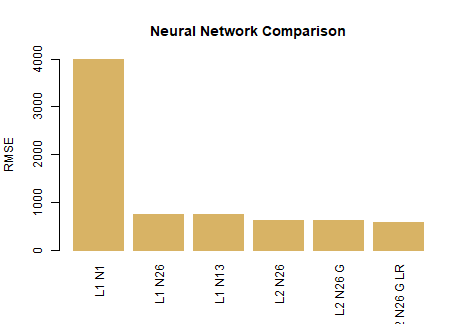
\includegraphics{Diamonds_PDF_files/figure-latex/NN Summary-1} \end{center}

As can be seen, the predictive performance of the neural networks can
vary a lot depending on the structure and parameters chosen. The
negative point in this method is the requirement of human input to
adjust the model to learn more precisely. Nevertheless, once the many
trials have been executed, the results are very positive for a good
predictive model.

\begin{figure}
\centering
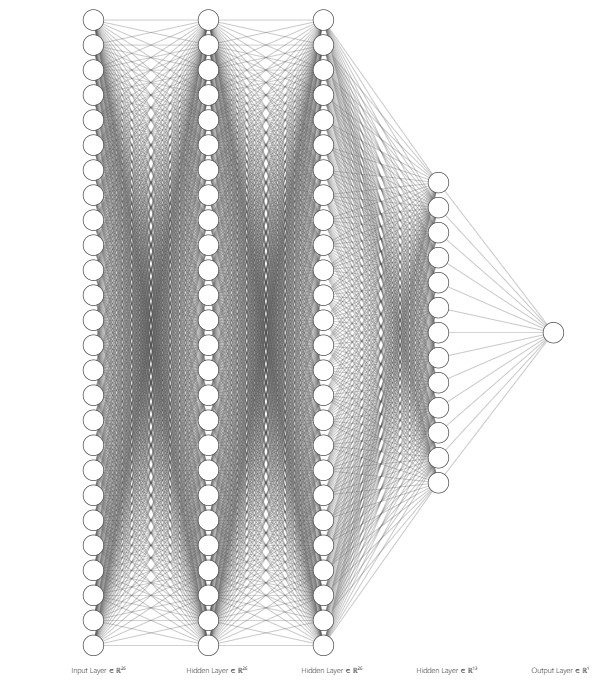
\includegraphics{NN_rep.jpeg}
\caption{Visual description of Neural Network}
\end{figure}

\hypertarget{ensembles}{%
\subsection{Ensembles}\label{ensembles}}

\hypertarget{overview-model-structure-and-analysis}{%
\paragraph{Overview, Model Structure and
Analysis}\label{overview-model-structure-and-analysis}}

`Ensemble methods is a machine learning technique that combines several
base models in order to produce one optimal predictive model.' The
simplest approach is to combine predictions from each method above that
had the best/lowest RMSE. To accurately compare models, the mean is
taken over the four models to compute the average predicted price and
find the error rates between the calculated price and real prices. As
the table reveals, the RMSE is \$588.34 which is pretty close to random
forests and the best neural network in terms of variance.

\begin{table}
\centering
\begin{tabu} to \linewidth {>{\raggedright}X>{\raggedleft}X>{\raggedleft}X>{\raggedleft}X>{\raggedleft}X>{\raggedleft}X}
\hline
  & ME & RMSE & MAE & MPE & MAPE\\
\hline
Test set & 25.80266 & 582.3353 & 306.1574 & -1.682175 & 8.448477\\
\hline
\end{tabu}
\end{table}

\begin{table}
\centering
\begin{tabular}{l|l|l|l|l|l}
\hline
  & ME & RMSE & MAE & MPE & MAPE\\
\hline
Multiple Linear Regression & 50.4 & 810.16 & 405.06 & -0.84 & 10.4\\
\hline
Random Forest & 2.97 & 577.63 & 289.51 & -1.4 & 7.24\\
\hline
k-Nearest Neighbor & 40.86 & 814.59 & 431.29 & -2.45 & 12.14\\
\hline
Neural Network & 8.98 & 577.08 & 322.95 & -2.03 & 10.23\\
\hline
Ensemble & 25.8 & 582.34 & 306.16 & -1.68 & 8.45\\
\hline
\end{tabular}
\end{table}

\hypertarget{model-performance-summary}{%
\section{Model Performance Summary}\label{model-performance-summary}}

In this section, we can see how the predicted price behaves with respect
to the real price, having used each of the methods and mapping per each
categorical variable. This helps see how each model compares with
regards to precision. The models with more precision are closer to a
diagonal line. As can be seen,

\hypertarget{predicted-price-vs-real-price-by-clarity}{%
\subsection{Predicted Price vs Real Price by
Clarity}\label{predicted-price-vs-real-price-by-clarity}}

\hypertarget{predicted-price-vs-real-price-by-color}{%
\subsection{Predicted Price vs Real Price by
Color}\label{predicted-price-vs-real-price-by-color}}

\begin{center}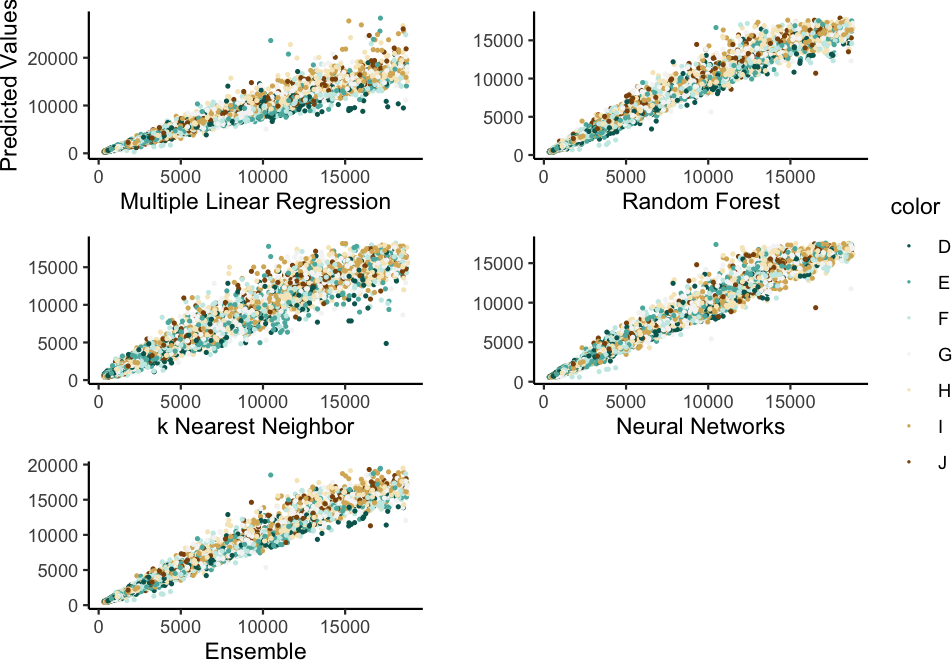
\includegraphics{Diamonds_PDF_files/figure-latex/Summ Color Plots-1} \end{center}

\hypertarget{predicted-price-vs-real-price-by-cut}{%
\subsection{Predicted Price vs Real Price by
Cut}\label{predicted-price-vs-real-price-by-cut}}

\begin{center}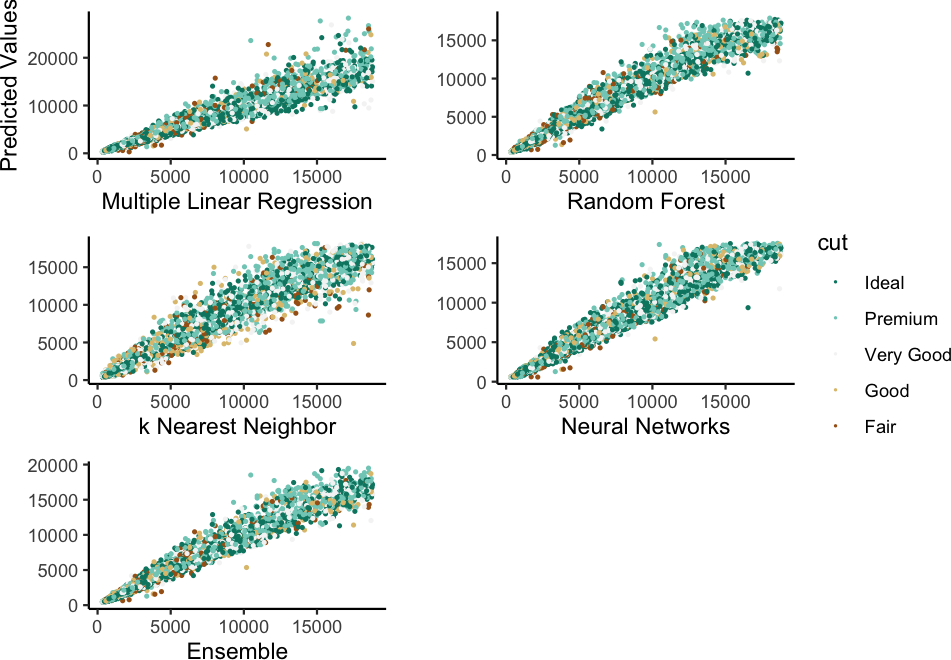
\includegraphics{Diamonds_PDF_files/figure-latex/Summ Cut Plots-1} \end{center}

\hypertarget{conclusions}{%
\section{Conclusions}\label{conclusions}}

\hypertarget{references}{%
\section{References}\label{references}}

EDA -
\url{https://r-graph-gallery.com/199-correlation-matrix-with-ggally.html}
and
\url{http://www.sthda.com/english/wiki/ggplot2-quick-correlation-matrix-heatmap-r-software-and-data-visualization}

k-NN -
\url{https://online.stat.psu.edu/stat508/lesson/k\#}:\textasciitilde:text=The\%20larger\%20k\%20is\%2C\%20the,Nearest\%20Neighbors\%20are\%20shown\%20below.\\
-
\url{https://www.analyticsvidhya.com/blog/2018/03/introduction-k-neighbours-algorithm-clustering/}

Regression Tree - Data Mining textbook -
\url{https://www.ibm.com/docs/en/db2-warehouse?topic=procedures-regression-trees}

Boosted Tree -
\url{https://towardsdatascience.com/introduction-to-boosted-trees-2692b6653b53}\\
-
\url{https://leonlok.co.uk/blog/decision-trees-random-forests-gradient-boosting-whats-the-difference/}

Bagging Tree -
\url{https://machinelearningmastery.com/bagging-and-random-forest-ensemble-algorithms-for-machine-learning/}

Random Forest - Data Mining textbook

Ensemble -
\url{https://towardsdatascience.com/ensemble-methods-in-machine-learning-what-are-they-and-why-use-them-68ec3f9fef5f}

Hardesty, Larry. 2017. {[}Explained: Neural Networks{]} MIT News.
(\url{https://news.mit.edu/2017/explained-neural-networks-deep-learning-0414})

\end{document}
